% LTex: language=pl
\section{Iteracje projektu oraz zmiany stanu wiedzy i wymagań}
Wymagania dotyczące docelowego systemu były pozyskiwane z poniższych źródeł:
\begin{itemize}
    \item Klient - Osoba dobrze zaznajomiona z funkcjami systemu, posiadająca powierzchowną wiedzę na temat jego implementacji oraz będąca w posiadaniu dostępu do serwera, na którym zostanie uruchomione docelowe rozwiązanie. Jest głównym źródłem wymagań funkcjonalnych systemu.
    \item Administrator STOS - Osoba znająca działanie systemu, umiejąca uruchomić system i rozwiązać istniejące problemy.
    \item Studenci - Bezpośredni użytkownicy systemu. Wymagania były zbierane poprzez ankiety, nieformalne rozmowy oraz doświadczenia autorów pracy.
    \item System STOS - Nieożywione źródło wymagań. Jest to istniejąca implementacja systemu, działająca na serwerach katedry algorytmów i modelowania systemów. Docelowe środowisko powinno  integrować części komponentów tego systemu, dostosować się do interfejsów komunikacyjnych i odzwierciedlać funkcjonalności obecnych modułów.
\end{itemize}
\indent Ze względu na uzależnienie platformy od odpowiedniej struktury systemu, ochronę algorytmu oceny oraz konieczność uzyskania zgody na publikację kodu przez jego autora, informacje o systemie były przekazywane dla naszego zespołu w sposób iteracyjny.
\newline \indent W pierwszej iteracji, datowanej na marzec 2024 roku, uzyskaliśmy informacje dotyczące istniejących problemów i ogólnego obrazu komponentów oraz ich roli. Ponieważ nie posiadaliśmy informacji na temat szczegółowego działania systemu, protokołów komunikacyjnych i środowiska docelowego, postanowiliśmy utworzyć przykładową wersję systemu, projektowaną z myślą o dynamicznie zmieniających się wymaganiach. Utworzony prototyp posiadał atrapę modułu oceniającego, serwisy Elasticsearch i Graylog pozwalające na gromadzenie i analizę logów, system zarządzający i gromadzący pliki oraz moduły pobierające, przekazujące i wykonujące pliki programów przesłanych przez studentów. Ze względu na szereg zalet konteneryzacji, wszystkie komponenty działały jako kontenery platformy Docker, zarządzane przez orkiestrator Kubernetes. Komunikacja pomiędzy serwisami odbywała się przez protokół http oraz kolejkę wiadomości RabbitMQ. By zbadać trudność implementacji, możliwość integracji zewnętrznych systemów oraz wydajność różnych technologii, komponenty zostały zaimplementowane w językach Java, Golang, Python oraz Rust. W celu zachowania spójnego formatu wiadomości i ich poprawnego przesyłania oraz odczytania zastosowano mechanizm serializacji Protobuf, opracowany i utrzymywany przez firmę Google.
\begin{figure}[!h]
	\begin{center}
		\resizebox{0.7\textwidth}{!} {
			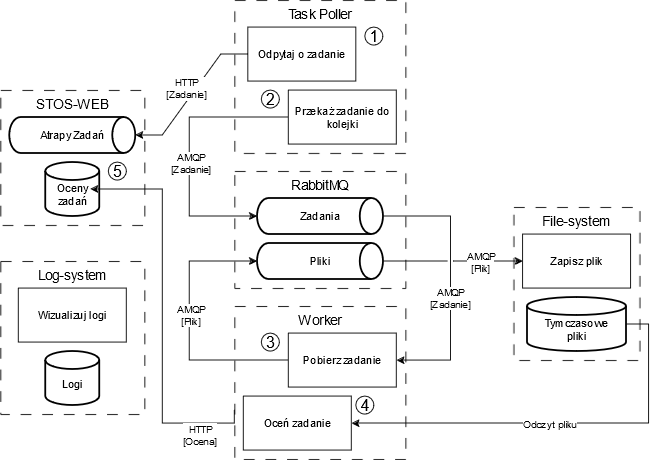
\includegraphics{img/1/i1_arch.png}
		}
		\caption[Architektura po pierwszej iteracji]{Diagram przedstawiający wysokopoziomową architekturę systemu, z uwzględnieniem komponentów, ich głównych funkcji oraz sposobu komunikacji. Źródło własne.}
	\end{center}
\end{figure}
\indent Druga iteracja projektu odbyła się w maju 2024 roku. Otrzymaliśmy wtedy informacje na temat szczegółowego działania komponentów w systemie oraz sekwencji operacji wykonywanych podczas procesu oceny zadania studenta. Zaznajomienie z komponentami pozwoliło nam na rozbudowę rozwiązania o mechanizm pamięci podręcznej. Kluczową otrzymaną informacją, był fakt działania modułu kompilującego w kontenerze na platformie Docker. W poprzedniej architekturze założyliśmy działanie całej strony serwerowej jako osobne serwisy uruchomione na tej samej maszynie wirtualnej, które w ramach docelowego systemu chcieliśmy przenieść do kontenera z naszym rozwiązaniem. Biorąc pod uwagę ścisłe powiązanie komponentów systemu i nowo otrzymaną informację, oznaczałoby uruchomienie zagnieżdżonego kontenera z modułem kompilującym w kontenerze z naszym rozwiązaniem. Znacząco podniosłoby to poziom skomplikowania, zarządzania systemem oraz detekcji awarii systemu.
\begin{figure}[!h]
	\begin{center}
		\resizebox{0.7\textwidth}{!} {
			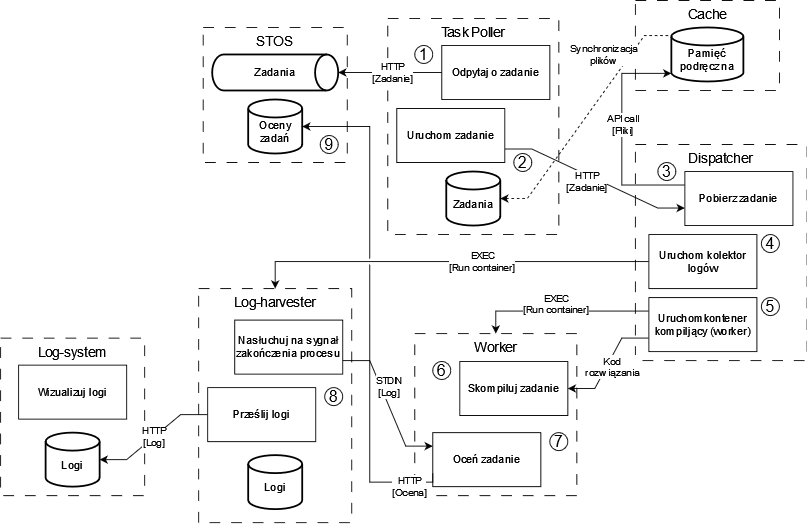
\includegraphics{img/1/i2_arch.png}
		}
		\caption[Architektura po drugiej iteracji]{Diagram przedstawiający wysokopoziomową architekturę systemu, z uwzględnieniem komponentów, ich głównych funkcji oraz sposobu komunikacji. Źródło własne.}
	\end{center}
\end{figure}
\indent W trzeciej iteracji projektu, która odbyła się w czerwcu 2024 roku, zostały szczegółowo wyjaśnione sposoby komunikacji między komponentami. Zdecydowaliśmy się na zmianę architektury systemu, w której pozostawiliśmy moduł kompilujący w dotychczasowej formie, utworzyliśmy serwis zarządzający instancjami tych kontenerów oraz serwis pobierający i przekazujący zadania. Całość będzie umieszczona na hipernadzorcy pierwszego stopnia, który jest trzecią alternatywą dla maszyn wirtualnych i kontenerów.
\begin{figure}[!h]
	\begin{center}
		\resizebox{0.7\textwidth}{!} {
			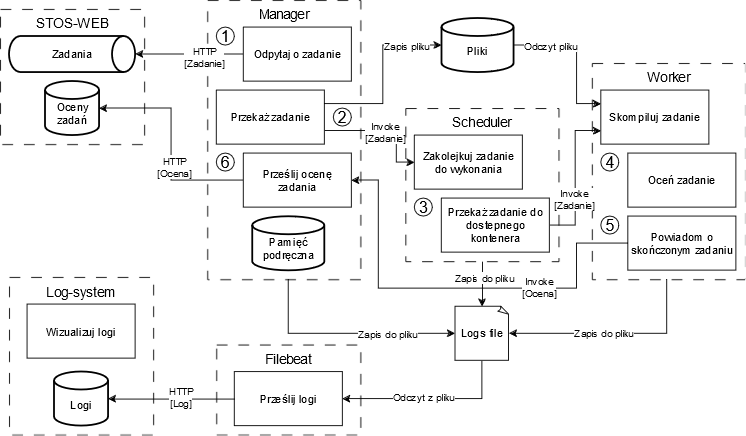
\includegraphics{img/1/i3_arch.png}
		}
		\caption[Architektura po trzeciej iteracji]{Diagram przedstawiający wysokopoziomową architekturę systemu, z uwzględnieniem komponentów, ich głównych funkcji oraz sposobu komunikacji. Źródło własne.}
	\end{center}
\end{figure}
\indent Czwarta iteracja odbyła się we wrześniu 2024 roku. Otrzymaliśmy wtedy informacje na temat docelowego systemu, na którym zostanie uruchomione tworzone rozwiązanie. Zostały również przekazane instrukcje do jego połączenia. Postanowiliśmy uruchomić i skonfigurować maszyny hipernadzorcy na serwerze. Skutkiem było uruchomienie środowisk deweloperskich, produkcyjnych oraz serwera logów. Sposób zarządzania został opisany w instrukcji, a poświadczenia zostały przekazane klientowi. Z racji nieuzależniania naszego rozwiązania od konkretnego systemu, nie wiązało się to ze zmianą architektury i implementacji. 
\begin{figure}[!h]
	\begin{center}
		\resizebox{0.7\textwidth}{!} {
			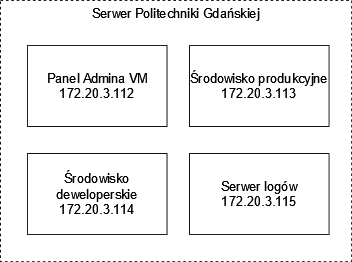
\includegraphics{img/1/i4_arch.png}
		}
		\caption[Maszyny wirtualne uruchomione na serwerze Politechniki Gdańskiej]{Diagram przedstawia uruchomione maszyny na serwerze, wraz z ich adresami. Źródło własne.}
	\end{center}
\end{figure}
\indent Ostatnia, piąta iteracja miała miejsce w październiku 2024 roku. Otrzymaliśmy wtedy wszystkie potrzebne pliki źródłowe systemu wraz z obrazem modułu kompilującego. Umożliwiło nam to na dogłębną analizę źródła i zrozumienie sposobu komunikacji między komponentami. Nowa wiedza wiązała się z koniecznością dostosowania naszego systemu do istniejącego. Zdecydowaliśmy się na zmianę działania systemu cache. Spróbowaliśmy również uruchomić system na naszych maszynach, a także przeprowadzić analizę jego zachowania z wieloma uruchomionymi instancjami modułu kompilującego jednocześnie. Szczegółowa architektura zostanie opisana w następnych rozdziałach.